\documentclass[conference]{IEEEtran}
\IEEEoverridecommandlockouts
% The preceding line is only needed to identify funding in the first footnote. If that is unneeded, please comment it out.
\usepackage{cite}
\usepackage{amsmath,amssymb,amsfonts}
\usepackage{algorithmic}
\usepackage{graphicx}
\usepackage{textcomp}
\usepackage{xcolor}
\usepackage{CJKutf8}
\def\BibTeX{{\rm B\kern-.05em{\sc i\kern-.025em b}\kern-.08em
    T\kern-.1667em\lower.7ex\hbox{E}\kern-.125emX}}
\begin{document}
\begin{CJK*}{UTF8}{gbsn}
\title{Difficult Text Analysis of Machine Translation Services base on
  Metamorphic Testing in Social Media}

\author{\IEEEauthorblockN{1\textsuperscript{st} Boyang Yan}
\IEEEauthorblockA{\textit{Research Center of Network and Communications} \\
\textit{Peng Cheng Laboratory}\\
Shenzhen, China \\
yanby@pcl.ac.cn}
\and
\IEEEauthorblockN{2\textsuperscript{nd} Given Name Surname}
\IEEEauthorblockA{\textit{dept. name of organization (of Aff.)} \\
\textit{name of organization (of Aff.)}\\
City, Country \\
email address}
\and
\IEEEauthorblockN{3\textsuperscript{rd} Given Name Surname}
\IEEEauthorblockA{\textit{dept. name of organization (of Aff.)} \\
\textit{name of organization (of Aff.)}\\
City, Country \\
email address}
\and
\IEEEauthorblockN{4\textsuperscript{th} Given Name Surname}
\IEEEauthorblockA{\textit{dept. name of organization (of Aff.)} \\
\textit{name of organization (of Aff.)}\\
City, Country \\
email address}
\and
\IEEEauthorblockN{5\textsuperscript{th} Given Name Surname}
\IEEEauthorblockA{\textit{dept. name of organization (of Aff.)} \\
\textit{name of organization (of Aff.)}\\
City, Country \\
email address}
\and
\IEEEauthorblockN{6\textsuperscript{th} Given Name Surname}
\IEEEauthorblockA{\textit{dept. name of organization (of Aff.)} \\
\textit{name of organization (of Aff.)}\\
City, Country \\
email address}
}

\maketitle

\begin{abstract}
  A huge amount of text comments are posted on different topics in Social Media
  every day. These topics are discussed in different languages by different
  language speakers. Most people encounter language and culture barriers when
  engaging in cross-language communication.
  Cross-language machine translation is useful for global integration.
  However, most of people are chosen human translation services.
  The reason is human translation services are accuracy and reliable compare
  with machine translation.
  Most research only focuses on ranking the quantity of machine translation
  services but little research has conducted on difficult translation text
  evaluation.
  This research explores what kind of text is difficult to translate for machine
  translation services base on movie comments data. It is useful for improve the quality
  of machine translation services to fill this research gap.
  This research is based on the Metamorphic Testing method to establish a
  testing model which using machine translation service translate original test
  dataset from one language to another language. After, using sentiment analysis
  tool to analyize original test dataset and translated datasets, the results
  should be same polarization (positive or negative). If the results are
  opposite polarization, that means this sentence is difficult for machine
  translation.
  As a result, people will able to use this testing model finding difficult
  sentences and doing specific optimiztion.
\end{abstract}

\begin{IEEEkeywords}
  Metamorphic Testing, machine translation, sentiment analysis, machine
  translation quantity testing, evaluation of machine translation services
  difficult, natural language
\end{IEEEkeywords}

\section{Introduction}
Machine translation services has been becoming more and more widely used, also
more and more popular. In especial, machine translation system has significantly increased
international trade\cite{brynjolfsson2018does}.
Most people encounter language and cultural barriers
during cross-language communication. There are lots of text and documents on different languages need
to translation every day. It would be impossible to translation the huge amount
of data generated manually. Nowadays, there are lots of machine translation
tools are available in the world, such as Google translation, Bing translation,
Yandex, Baidu translation and Youdao translation and so on. In this research,
only compare and evaluation Google translation, Yandex translation and Baidu
translation difficults. Those three translation tools are typical and the most
widespread to used. Google translation tool come from American, Yandex come from
Russia, and Baidu come from China. This three tools all come from the top three
powerful country. Accounting to Pesu said machine translation
tools can product better results on European languages compare with Asian
language \cite{pesu2018monte}. So, Chinese to English translation tool is the main
kind of translation languages to analysis translation difficults in the paper.
Evaluation of machine translation services difficults usually need language
expert, who need well-known both languages, to participate. However, language
expert also involves human emotional judgment. Automatic assessment human
language is naturally difficult because of without a test oracle \cite{zhou2016metamorphic}.
In this paper, achieving a testing modle to automatic assessment
without language expert. Metamorphic testing(MT) is one of property-based
software quality testing method, which alreadly be appoved effective for
addressing the oracle problem, such as testing the quality of search engine
and the quality of Unmanned Aerial Vehicle(UAV) flight control application and so on.
Therefore, decideing metamorphic testing to find machine translation services
difficults in non-oracle sitation.
And more specifically, this research raise two questions.
\begin{itemize}
  \item Q1: What is current sitation of the quantity of Chinese to English
    machine translation?
  \item Q2: What is current machine translation difficults between Chinese and English?
\end{itemize}

The rest of paper is organized as three parts. Firstly, domonstration the
quantity of Chinese to English translation services, which are Google
translation, Yandex translation and Baidu translation. This part addresses Q1.
secondly, describtion testing model about finding the difficults of machine
translation.
Thirdly, analyzes the experimental results and discussion. This part will
answer Q2.

\section{Background}
\subsection{Metamorphic Testing}
Metamorphosis Testing (MT) is a method for generating test cases, as well as test
results verification \cite{zhou2017introduction}. The most importance component is the metamorphic
relation (MR) \cite{chen2003fault}. MR is the target application's necessary
properties of function in relation to multiple inputs and their expected outputs.
MT has been researched through more and more researchers constantly strive
toward and adopted by industries and organizations such as Adobe, NASA and the
National Institute of Standards and Technology \cite{zhou2018metamorphic}.
In software testing research field, an incapacity to decide, software product
the correct output, is called the oracle problem \cite{brown2018metamorphic}.
This usually means cannot provide exact correctness reference data. such as,
machine translation. Huge and complexity systems, does not have
reference data for proving function's correctness, is very common.
When people want to assess the the accuracy of $\sin$ function. For example, $\sin(2.7)$ is very difficult to
make a correctness judgment from mathematics aspect. If using Metamorphic
Testing method to testing $\sin$ function will reduce computational costs and
more efficient. There is a testing procedures' example for $\sin$ function.
\begin{enumerate}\label{itm:procedures}
\item set a Metamorphic Relation: such as $$\sin(\alpha) = \cos(\frac{\pi}{2} - \alpha)$$
\item $\sin(2.7)$ and $\cos(\frac{\pi}{2} - 2.7)$ should have same output, if the
  outputs are different. We can say, this MR have been break, maybe the failure
  have been detected.
\end{enumerate}
However, when using \ref{itm:procedures}'s testing procedures. Someone maybe
ask, $\cos$ function also not reliable, how can use a unreliable function to
test another function's correctness. There have the boundedness. However, both
function have got failures at same time, that is small probability event.
\subsection{Sentiment Analysis}
Sentiment analysis is a part of text data mining. The aim of sentiment analysis
is to determine the attitude of speakers or writers with respect to particular
topics or the overall contextual polarity or emotional reaction to a text
document. It is usually equated with opinion mining, which involves the use of
natural language processing and machine learning to ascertain the possibility of
positive or negative opinions \cite{yadollahi2017current}. Sentiment analysis is useful for analyzing a
huge amount of data relating to personal opinions. It can be used in an
e-business context. For example, business managers can analysis customers’
attitudes, as to whether they like or dislike their product or service. Also,
government can use sentiment analysis to analyze citizen perspectives.
In this paper, we will using Google Sentiment Analysis tool to prove the the
quantity of Machine Translation. The details of Testing Modle will talk in \ref{testingModle} .

\section{domonstration the current quantity of Chinese to English translation
  services} \label{currentQuantity}

\subsection{Test Sample}
All of test sample came from Douban\footnote{Douban Website:
  https://www.douban.com/}, one of biggest social networking service
platforms in China. This social website attracts more than one hundred million
active visitors per month, and has amassed over sixty-five million registered
users \cite{doubanStat}. We then employ the Douban public Application Programming Interfaces
(APIs) to access Chinses-written comments. A typical data structure of harvested
comment is shown as a tuple: [Rating, Raw comments]. Totally, comments have got
46180 in the corpus. User rating total have 5 groups, which are 10, 20, 30, 40
and 50, from negative to positive.
The test sample distribution diagram on below.
\begin{figure}[h]
  \centering
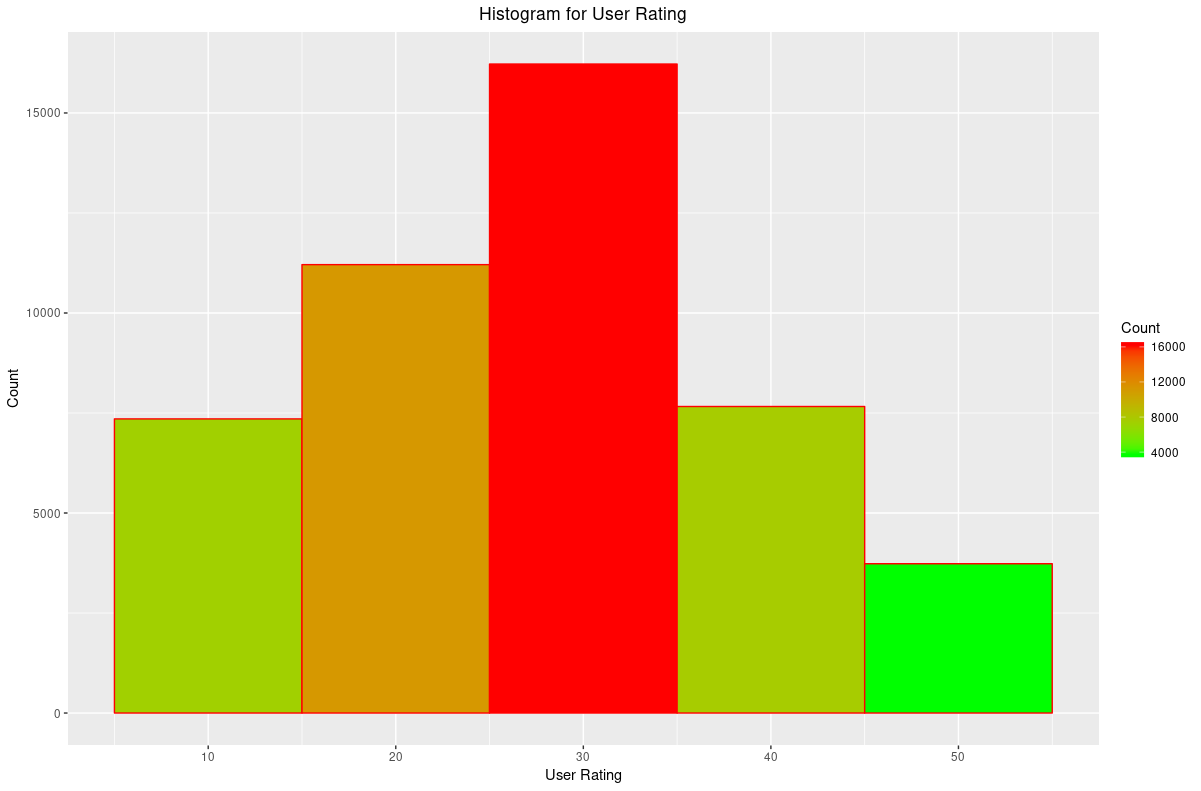
\includegraphics[width=0.3\paperwidth]{./img/ratingHis.png}
\caption{User Rating Histogram}
\label{fig:userRatingHistogram}
\end{figure}
As you can see, the majority of comments allocate on rating 30. In addition,
there have got more negative comments compare with positive comments.

\subsection{Testing procedures} \label{testingModle}
\begin{figure}[h]
  \centering
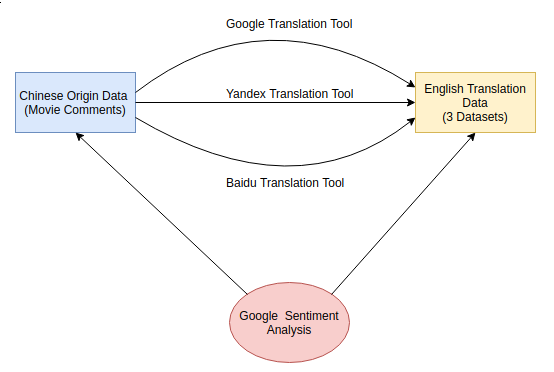
\includegraphics[width=0.35\paperwidth]{./img/model.png}
\caption{Testing Procedures}
\label{fig:testingProcedures}
\end{figure}
One the below, will explain more details for figure \ref{fig:testingProcedures}.

\begin{enumerate}
  \item using three of machine translation services to translate Chinese
    original movie comments to English translated movie comments.
    $$P_{(Origin Data)} \rightarrow P^{\prime}_{(Google Translation)}$$
    $$P_{(Origin Data)} \rightarrow P^{\prime}_{(Yandex Translation)}$$
    $$P_{(Origin Data)} \rightarrow P^{\prime}_{(Baidu Translation)}$$
  \item Using Google sentiment analysis tool to analysis $P_{(Origin Data)}$,
    $P^{\prime}_{(Google Translation)}$, $ P^{\prime}_{(Yandex Translation)}$ and $
    P^{\prime}_{(Baidu Translation)}$. Google sentiment analysis APIs will get 2
    values, which are Score and Manitude. The range of Score is between -1 and
    1. If Score more close to 1 means this movie comment more positive, as well
    as, if Score more close to -1 means this movie comment more negative. In
    this paper, we have not analysis Manitude, which for distinction mix and neutral.
  \item\label{itm:testingProcedure3} Using user rating values (10, 20, 30, 40 or 50) to check Google
    Sentiment Analysis(SA) results $P_{(Origin Data)} $ is True or False. For
    example, user rating = 10 and Google Chinese SA score between -1
    and -0.6 (mean True) user ranking = 10 and Google Chinese SA score bigger
    than -0.6 (mean False). The decideing True table on below.\\
     \begin{table}[h]
      \caption {The Range of Score: True/ False}
     \begin{center}
      \begin{tabular}{|c|c|c|c|}
        \hline
        user rating & Google SA score & True/False \\
        \hline\hline
        10 & $[ \, -1, -0.4 ] \,$ & True \\
        \hline
        20 & $[ \, -0.8, 0 ] \,$ & True \\
        \hline
        30 & $[ \, -0.4, 0.4 ] \,$ & True \\
        \hline
        40 & $[ \, 0, 0.8 ] \,$ & True \\
        \hline
        50 & $[ \, 0.4, 1 ] \,$ & True \\
        \hline \hline
        10 & $( \, -0.4, 1 ] \,$ & False \\
        \hline
        20 & $[ \, -1, -0.8) \,$ & False \\
        \hline
        20 & $( \, -0.8, 1] \,$ & False \\
        \hline
        30 & $[ \, -1, -0.4) \,$ & False \\
        \hline
        30 & $( \, 0.4, 1] \,$ & False \\
        \hline
        40 & $[ \, -1, 0) \,$ & False \\
        \hline
        40 & $( \, 0.8, 1] \,$ & False \\
        \hline
        50 & $[ \, -1, 0.4) \,$ & False \\
        \hline
        \hline
      \end{tabular}
    \end{center}
  \end{table}

    As you can see, the Google SA score ranges have got some overlap because
    overlap can decrease the results, machine translation evaluation
    correctness, influence by the accuracy of Google Sentiment Analysis tool.
  \item Using those True or False values as vector combining with Google English
    SA scores (based on $P^{\prime}_{(Google Translation)}$), Google English SA
    scores (based on $ P^{\prime}_{(Yandex Translation)}$) and Google English SA
    scores (based on $P^{\prime}_{(Baidu Translation)}$) draw 3 Receiver operating
    characteristic (ROC) graphics and 3 Precision-recall curves (PRC) graphics.

    ROC curve is often used in evaluation the clinical performance of a
    biochemical test \cite{zweig1993receiver}. The ROC curve is based on a
    series of different binary
    classifier with the true positive rate (sensitivity) as the Y-axis and the
    false positive rate (1-specificity) as the X-axis \cite{ROC}. The traditional
    evaluation must be divided into two categories, and then statistical
    analysis is performed. The ROC curve is different from the traditional
    evaluation method. Instead, an intermediate state is allowed. The test
    results can be divided into multiple ordered classifications then
    statistically analyzed. However, visual interpretation and comparisons of
    ROC curves based on imbalanced data sets can be misleading. An alternative
    to a ROC curve is a precision-recall curve (PRC). PRC might be a better
    choice for imbalanced datasets \cite{davis2006relationship}.
    This graphic show those three of machine translation tools all achieve poor
    translation results.
\begin{figure}[h]
  \centering
    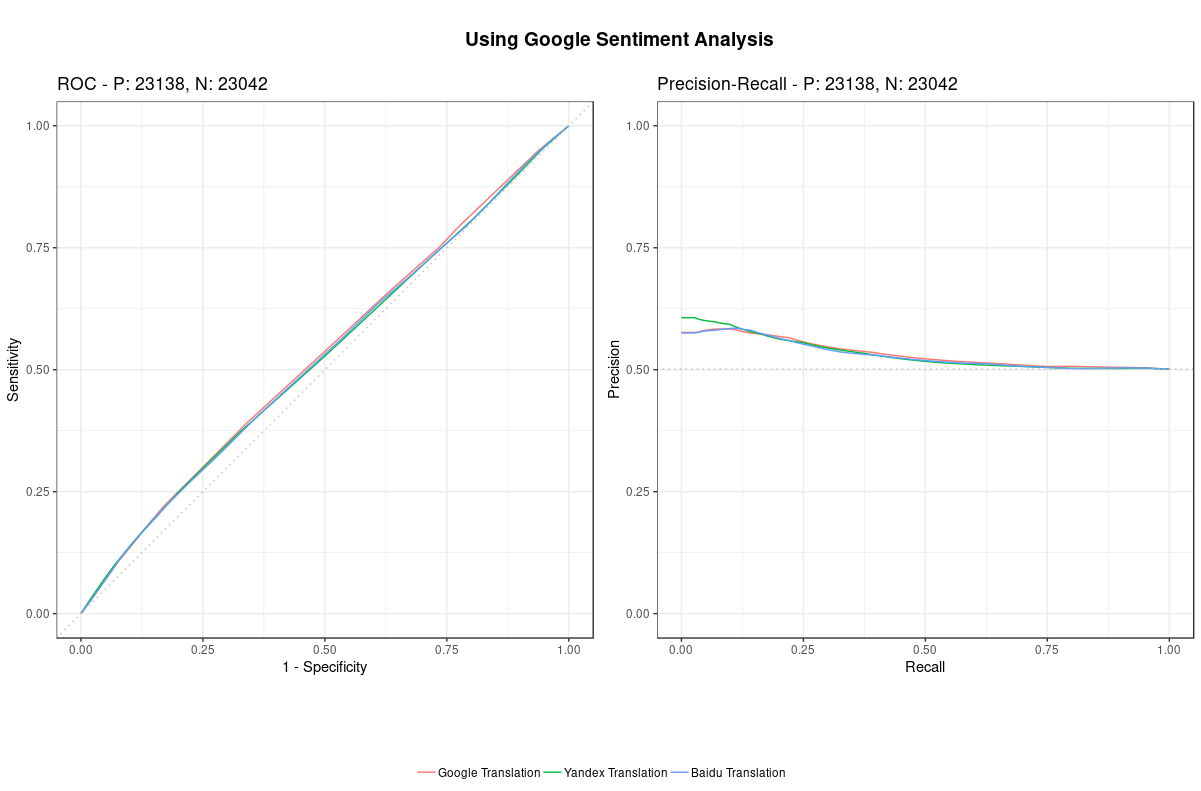
\includegraphics[width=0.35\paperwidth]{./img/ROCandPRC.png}
\caption{ROC and PRC graphics}
\label{fig:ROCandPRC}
\end{figure}
  \item Calculate Area Under The Curve (AUC) values for ROC and PRC.
    \begin{table}[h]
      \caption {Google Translation}
    \begin{center}
      \begin{tabular}{|c|c|}
        \hline
        Curve Types & AUCs \\
        \hline\hline
        ROC & 0.5307797 \\
        \hline
        PRC & 0.5328503 \\
        \hline
      \end{tabular}
    \end{center}
  \end{table}
   \begin{table}[h]
     \caption {Yandex Translation}
     \begin{center}
       \begin{tabular}{|c|c|}
         \hline
         Curve Types & AUCs \\
         \hline\hline
         ROC & 0.5251734 \\
         \hline
         PRC & 0.5322736 \\
         \hline
       \end{tabular}
     \end{center}
   \end{table}
  \begin{table}[h]
    \caption {Baidu Translation}
    \begin{center}
      \begin{tabular}{|c|c|}
        \hline
        Curve Types & AUCs \\
        \hline\hline
        ROC & 0.5258386 \\
        \hline
        PRC & 0.5302736 \\
        \hline
      \end{tabular}
    \end{center}
  \end{table}\\
  The AUC is between 1.0 and 0.5. The better diagnostic effect will be close to
  1. The ranking of accuracy is show on Table: \ref{accuracyJudgment}\\\\
  \begin{table}[h]\label{accuracyJudgment}
    \caption {ROC and PRC accuracy judgment}
     \begin{center}
       \begin{tabular}{|c|c|}
         \hline
         AUC value & Accuracy \\
         \hline\hline
         $[ \, 0.5, 0.7] \,$ & lower accuracy \\
         \hline
         $[ \, 0.7, 0.9] \,$ & certain accuracy \\
         \hline
         $[ \, 0.9, 1] \,$ & higher accuracy \\
         \hline
       \end{tabular}
     \end{center}
   \end{table}
  When AUC=0.5, it means that the diagnostic method is completely ineffective
  and has no diagnostic value \cite{baiduROC}.
\end{enumerate}
  \subsection{Current Translation Tool Results Analysis}
  In the testing Procedures \ref{itm:testingProcedure3}, which is the judgment of Google Chinese
    Sentiment Analysis(SA) results is True or False, there are totally have find
    23042 of true value, as well as 23138 of false value. Alought the dataset is
    looks balanced, ROC diagram can be trusted. The ranking of machine
    translation services' quantity are NOT reliable. The reason is three of
    translation services have lower accuracy. In another word, working not
    properly correct. However, there are still have the ranking of machine
    translation services' quantity on the below.
\subsubsection{For ROC AUCS}
\textbf{It shows Google Translation tool better than Baidu Translation tool better than Yandex Translation tool}
\subsubsection{For PRC AUCS}
\textbf{It shows Googl Translation tool better than Yandex Translation tool better than Baidu Translation tool}

\section{finding the difficults of machine translation}
\subsection{Testing procedures}
The first two step is same with, showing the current quantity of Machine
Translation Tools in Section \ref{currentQuantity}. Which are get translated
datasets and sentiment analysis for 4 datasets(Chinese Origin dataset, Yandex
translation dataset, Google translation dataset and Baidu translation dataset).
The only different is filting all of opposite polarization (very positive or
very negative) datasets and create three of Metamorphic Relation (MR).
\subsubsection{MR1}
$$SA_{(Origin Data)} \approx SA^{\prime}_{(Google Translation)}$$
\subsubsection{MR2}
$$SA_{(Origin Data)} \approx SA^{\prime}_{(Yandex Translation)}$$
\subsubsection{MR3}
$$SA_{(Origin Data)} \approx SA^{\prime}_{(Baidu Translation)}$$
\subsection{Analysis}
MR1, MR2 and MR3 have got failures decideing by one side greater than 0.7 and
another side smaller than -0.7. In this paper, using veen diagram for show
failures distribution.
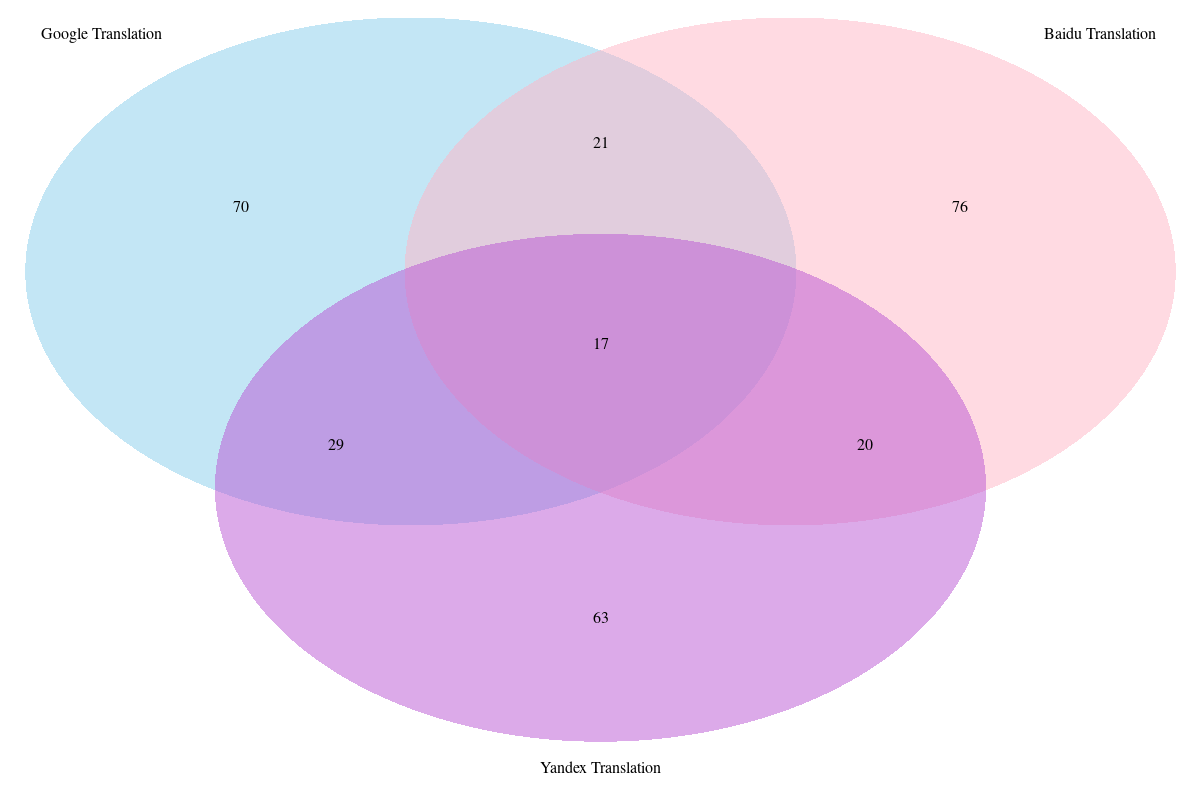
\includegraphics[width=0.35\paperwidth]{./img/veen.png}

  \begin{table}[h]
    \caption {Translation Failures Distribution}
    \begin{center}
      \begin{tabular}{|c|c|}
        \hline
        Types & Number Of Failures \\
        \hline\hline
        google Translation & 137\\
        \hline
        Yandex & 129 \\
        \hline
        Baidu & 134 \\
        \hline
        $Google \cap Baidu$ & 38 \\
        \hline
        $Google \cap Yandex$ & 46 \\
        \hline
        $Yandex \cap Baidu$ & 37 \\
        \hline
        $Yandex \cap Baidu \cap Google$ & 17 \\
        \hline
      \end{tabular}
    \end{center}
  \end{table}\\


\subsection{Language Analysis}
翻译质量评价总结

主要问题在于以下几个方面:
第一、词汇问题:
Google translation:
1.Error points语序混乱,滥用词汇和用法不正确,顺序混乱,Missing vocabulary,Improper selection of words,The words are raw.
例如sententChinese“2013最后一场电影 就为恶心画一句号吧”,Sentent
GoogleTranslation“Let's take a look at the last movie of 2013.”The translation
is fragmented and incomplete,The wrong translation of words refers to the
emotional color and stylistic misinterpretation of words。 应翻译为“ The last
movie is a full stop for nausea in 2013.”

3 of then
比如,“这片子真垃圾 就最后一点看起来比较有新意”GoogleTranslation和YandexTranslation都翻译了原文“ innovative”。但baiduTranslation用了“new”。

google and baidu
2.Translation error with noun ,misuse and incorrect usage,Sequential chaos。例如sententChinese“想法不错,可惜节奏把握的不好”,baiduTranslation“The idea is good, but the rhythm of the rhythm is not good”.应翻译为”The idea is good, but it is pity that the rhythm is not good”.


all 3
没那么烂,比春晚好
3.Misinterpretation of professional terms and literary terms.比如“春晚”GoogleTranslation准确翻译为 “Spring Festival Gala”,但是YandexTranslation错误地翻译为“show ”。错误地翻译baiduTranslation用了“spring”。

********************************************************************************
4.望文生意
google only
比如“片子没你们说的那么难看”GoogleTranslation翻译为“the film did not you say so ugly”这个“难看”不可翻译为“ugly”,应该翻译为“Boring”;再如,“冯导的电影是非真多”不可以翻译成“Feng's film is not true”,应翻译为“there are a lot of dispute in Feng's film ”。Translation error with noun这个“是非”不可翻译为“is not true”和“right and wrong”,应翻译为“dispute”.

5.目标语背景知识缺乏
google only
An expression habit that is not suitable for English,Statement is not smooth,
比如GoogleTranslation当提到“戴高帽子”时,不可翻译为“wear that tall hat”,应翻译为“Flattery”.

6.词语的感情色彩、语体误译。
all 3
Word color misinterpretation refers to the emotional color of words, stylistic
misinterpretation.原文“很写实,已经不是电影了,明明就是戏剧化的焦点访谈节目,披
露这个社会这个世界和一些人的嘴脸和生活…”中“嘴脸”这个词,三个翻译软件都翻译为
“face”根据文中的原意,应该改译“Ugly face;Lewd appearance.”
!!!!!!!!!!!!!!!!!!!!!!!!!!!!!!!!!!!!!!!!!!!!!!!!!!!!!!!!!!!!!!!!!!!!!!!!!!!!!!!!!!!!!!!!!!!!!!!
第二、Grammatical errors
1.Sequence disorder、Improper location of attributive、Improper position of adverbial (improper location of time adverbial, place adverbial and other adverbial)、Improper location of clauses.Ingredients are incomplete.The subject is incomplete, the predicate is incomplete, the attributive is incomplete, the adverbial is incomplete, the object is incomplete, etc.

3 all
比如,原文“明明是搞笑片最后弄成了教育片”baiduTranslation翻译为“It's a funny movie that finally makes an education film”.“that”improper collocation of the main guest Illogical.应该翻译为“Obviously it is a comedy,but it  made into education films finally”;
GoogleTranslation翻译为“Think of a bad movie, but did not expect to be able to
rot to this point”;YandexTranslation都翻译了原文“ Thought is a bad film, just
didn't think it could be rotten to the point ”。baiduTranslation用了“That is a
bad film, but did not expect to come to this rotten”。三种翻译工具都共同存在的问
题是“I do think the it is a bad moive,but I did not expect to be able to rot to
this point”Sequence disorder and Ingredients are incomplete(The subject is
incomplete);

google only
原文“为贪污腐败和商业大俗片辩护的一部元素太多深度太浅的电影”,GoogleTranslation原译“An  element too deep and too shallow to justify corruption and commercial tyranny.”改译“it is a film with too shallow meaning and max lot of element for defend corruption and commercial tyranny”


google only
2.句子结构方面问题.句子成分残缺不全,语序混乱.
GoogleTranslation“几小杯葡萄汁,很不新鲜”,错误地翻译为“A few small cups of
grape juice, very fresh”,应该翻译为“A few small cups of grape juice, it is not
very fresh”;

GoogleTranslation原句“个人意见,如果想看的同学们可以去买各种打折团购
之类的票,因为真心不值票价”,错误地翻译为“Personal opinion, if you want to see
the students can buy all kinds of discount buy tickets, because the true
worthless fare”,应该翻译为“Personal opinion, if students who want to see the
film  can buy all kinds of discount tickets, because it is worthless fare”.

baiduTranslation原句“前半段还不错~讽刺的意味很重,最后的道歉有点多余了”,错误地
翻译为“The first half was good - the irony was very heavy, and the last apology
was a little redundant”.“-”Improper location of clauses.和“and”The misuse of
conjunctions应该翻译为“The first half was good with heavy  irony,but the last
apology was a little redundant”.


3.句子结构方面问题.表示因果关系不清
GoogleTranslation原文“我是个温和的人,实在是不忍心给太少的星。。。”原译“I am a
gentle person, and I really do not have the heart to give too few stars. . .”改
译“I can not ignorant conscience to give too few stars,because I am a gentle
person”.An expression habit that is not suitable for English,Statement is not
smooth。

GoogleTranslation原文“为贪污腐败和商业大俗片辩护的一部元素太多深度太浅的电影”,原
译“An  element too deep and too shallow to justify corruption and commercial
tyranny.”改译“it is a film with too shallow meaning and max lot of element for
defend corruption and commercial tyranny”.

\section{Conclusion}
Google Translation, Yandex Translation and Baidu Translation are basically
fluent and understandable. However, all of three translation services have get the
individual words are not properly selected and the language expression does not
conform to the natural speaking. Some of the mistranslations almost overlap.

\section{analysis of causes}
Although the length of the movie commentary sentences is short, the vocabulary
is not difficult and the sentences' structure seems simple, there have got
lots of colloquial speech and many of words are not formal, which is the main
reason for the low quality of translation results. Lots of compound
sentence is hidded. It is more difficult for intelligent machines translation
services.

\section{future work}
Due to the differences way of thinking between Chinese and English languages. In
addition, cultural differences and the limitation of translation corpus.
Machine translation tools have serious language problems. Machine translation
researchers must be work with linguistic researchers, who should be paid more
attention to the corpus, lexical analysis and grammatical analysis.

\section{consideration and suggestion}


\bibliographystyle{IEEEtran}
\bibliography{library}
\end{CJK*}
\end{document}
